%! Author = florian
%! Date = 30.10.22

% Preamble
\documentclass[10pt,journal]{IEEEtran}

% Packages
\usepackage{amsmath}
\usepackage[english]{babel}
\usepackage{url}
\usepackage{listings}
\usepackage{libertine}
\usepackage{libertinust1math}
\usepackage[T1]{fontenc}
\usepackage{hyperref}
\usepackage{glossaries}
\usepackage[a4paper, total={6in, 9in}]{geometry}

%Glossary
\makeglossaries
\newglossaryentry{EO}{
    name=EO,
    description={An OOP paradigm}
}

\newglossaryentry{OOP}{
    name=OOP,
    description={A programming paradigm that is centered around objects}
}

\newglossaryentry{API}{
    name=API,
    description={An application programming interface
    allows two applications or a programmer and a library to talk to each other},
    plural={APIs}
}

\title{Elegant Objects: A OOP Paradigm}
\author{Florian Weingartshofer}
\date{November 3, 2022}

% Document
\begin{document}
    \maketitle

    \selectlanguage{english}

    \section{Introduction}\label{sec:introduction}


    \section{Principles}\label{sec:principles}
The elegant objects paradigm is based on eleven principles.
They will be discussed in this chapter, along with some examples and some limitations of the principles.

In the elegant objects an object is viewed differently than in \Gls{OOP}.
An object should never be some kind of data holder, like a struct in C\@.
An object has to strictly encapsulate its members, which forces developers to use the tell-dont-ask principle.
In elegant object the object is often compared to a living being and should therefore be respected.\cite{tell-dont-ask-martin-fowler,elegant-objects}

\subsection{No Null}\label{subsec:no-null}
Null references has been described as the billion-dollar mistake multiple times\footnote{\url{https://www.infoq.com/presentations/Null-References-The-Billion-Dollar-Mistake-Tony-Hoare/}}.
All references have to be checked for null and code bases become polluted by null checks.
The alternatives to null would be to use in some cases an iterator, like c++ does when working with collections, or to define empty objects of a class.
For example, if an employee cannot be retrieved from a database, an empty employee object is returned.
These empty objects have default values for some methods, but will throw an exception for others.

Another more modern alternative is to use \texttt{Optional} in Java or nullable types in programming languages that support it, like typescript or c\#.
This forces the user of a library to check if the object is present and react accordingly.
For example, the ArrayList\ \ref{fig:optional-usage} that was implemented alongside this paper uses this approach, if the first element of the list is requested.
The use of Optional forces the user to react to null values, by checking if a value is present in the Optional.

\begin{figure}[h]
    \caption{Optional Usage in ArrayList}
    \lstinputlisting[language=Java,basicstyle=\tiny,label={lst:optional-usage},firstline=97,lastline=102]{../java/at/fhooe/collections/ArrayList.java}
    \label{fig:optional-usage}
\end{figure}

Another solution is to throw an exception.
This can be used if an operation should not result in a null reference.

Null values are often used in objects that are lazy loading and therefore mutable.
The subsection\ \ref{subsec:no-mutable-objects} describes the reason to use immutability.
The main reason why lazy loading is bad, is that it is a bad practice in \gls{OOP}.
An object will then also be responsible for performance problems, e.g.\ the object will have more than one responsibility,
the original intend for the object and lazy loading.
This is a clear violation of the single responsibility principle.
By using a caching solution paired with aspect orientated programming, it is possible to move the performance problem to a caching library, like Google Guava.\cite{elegant-objects}

\subsection{No Code in Constructors}\label{subsec:no-code-in-constructors}
Code in constructors is a common practice in \gls{OOP}, but it violates some best practices.
First, doing calculations in a constructor changes the meaning of the new keyword.
It turns the new operation into a static operation, which also should not be used, since it is imperative programming and not \gls{OOP}.
In imperative programming, function does some calculations and returns its result, but in \gls{OOP} the calculations are delayed until they are needed.

Furthermore, doing calculations in the constructor can lead to unexpected side effects for the user.
For example, if it would be uncommon to read data from a database in a constructor.
Either the calculation has to be done before constructing the new object or by calling a method on the new object.
By belaying the calculations to the last possible point, it assures that no result is calculated that is not needed.\cite{elegant-objects}

\subsection{No Getters and Setters}\label{subsec:no-getters-and-setters}
Getters and setters should not be used.
They are an inherent risc to data encapsulation.
When using setters properties can be exposed and the state of the object is altered from the outside.
Simply, the object cannot encapsulate its own state.\cite{encapsulation}
Getters and setters expose implementation details.
If the implementation of an object changes, the getter will also change and in consequence, programs relying on the getter will break.

Another reason against getters and setters is ``Tell, don't ask'', this means instead of asking an object for information, to tell an object to calculation on the information it already has and then return the result.
By doing this an object is not burdened with the internals of another object.\cite{tell-dont-ask}

One reason why getters and setters are so widespread is because objects are used as data holders.
This is a common misconception from C and other imperative programming languages.
Instead of asking for the information from an object, the user should think how the object can calculate a result that is useful.\cite{elegant-objects}

\subsection{No mutable Objects}\label{subsec:no-mutable-objects}
A object is immutable if its state cannot be modified after its creation.
The string implementation is an example for immutable objects.
There are several reasons to prefer immutable objects to mutable ones.\cite{elegant-objects}

\begin{itemize}
    \item Immutable objects are thread-safe, as they cannot change the state after creation
    \item Immutable objects are easy to construct and to test
    \item It is easy to avoid temporal coupling
    \item Immutable objects are side effect free
\end{itemize}

\subsubsection{Thread Safety}
Since immutable objects cannot change their state, all threads accessing the object will have the correct and most recent state of the object.
This means multiple threads can access the same object at the same time, without any clashes.

\subsubsection{Construction and Testing}
Immutable objects are easy to construct, since all members have to be initialized in the constructor not later.
Testing them is also closely related with\ \ref{subsubsec:avoid-temporal-coupling}, since it is easy to construct them and when they are constructed they are ready to use.

\subsubsection{Avoid Temporal Coupling}\label{subsubsec:avoid-temporal-coupling}
Temporal coupling is, when multiple methods have to be called in a particular order or else the result would not be correct.
A simple example is the \texttt{init}-method, that can be seen in some code bases.\cite{temporal-coupling}

Figure\ \ref{fig:temporal-coupling} is a simple example of what temporal coupling looks like.
Another example would be the Java \texttt{HttpUrlConnection} class\footnote{\url{https://docs.oracle.com/javase/8/docs/api/java/net/HttpURLConnection.html}}.

\begin{figure}[h]
    \caption{Simple Temporal Coupling}
    \begin{lstlisting}[language=Java,basicstyle=\tiny,label={lst:temporal-coupling}]
        class DatabaseConnection {
            DatabaseConnection(String con) {/*...*/}
            void init() {} // Open Connection

            // Send Sql query
            // throws if init is not called
            Object send(String query) {}
        }
    \end{lstlisting}
    \label{fig:temporal-coupling}
\end{figure}

Immutable objects make it impossible to depend on temporal coupling, since calling any method will not change the state of the object.
Temporal coupling only works if the state can be changed.\cite{elegant-objects}

\subsubsection{Avoid Side-Effects}
A method with side effects is a method that modifies the state of an object or does something else beyond its scope.
Important is that any method calling a method with side effects is also a method with side effects.
For example, logging or writing to a file.
Another example and bad practice is the modification of incoming parameters\footnote{\url{https://softwareengineering.stackexchange.com/questions/245767/is-modifying-an-incoming-parameter-an-antipattern}}.

Since the state of immutable objects cannot be modified, they are side effect free.
Obviously, some side effects are necessary, like writing to a database or logging.\cite{elegant-objects}

\subsection{No Objects with Names ending with -ER}\label{subsec:no-objects-with-names-ending-with--er}
A object with a name ending with -er indicates that it is a collection of procedures.
Because these procedures are in a class or object, does not mean this is object orientated programming.

The ``ER''-postifx is not the only naming convention that indicates that a class is a collection of procedures.
Other examples are ``-Utils`` and ''-able``

Instead of using these naming conventions, classes need to be refactored, that the name represents what the class is and not what it does.
For example, instead of it being named a \texttt{HuffmanEncoder}, it is named \texttt{HuffmanEncoding} with an \texttt{encode} method.\cite{er-postfix,elegant-objects}

\subsection{No static Methods}\label{subsec:no-static-methods}
A static method is just a procedure, therefore not part of \gls{OOP}.
It does not matter if the static method is private or public.
A static method should either be refactored in its own class, for reusability or removed.

For example, \texttt{java.lang.Math} is just a collection procedures for math functions.
Using any \texttt{Math} procedure tightly couples the code with \texttt{Math}.
Static methods do not have to conform to an interface.
Therefore, it is hard to change the implementation of \texttt{Math}.
Instead, there should be classes that implement parts of the math library accordingly.
That way, it is simple to change implementations.
For example, adding a caching mechanism to the implementation.\cite{elegant-objects}

\subsection{No instanceof, type casting, or reflection}\label{subsec:no-instanceof-type-casting-or-reflection}
\texttt{instanceof} discriminates against objects, by saying they should adhere to one contract, aka an interface or class, and then casting them to another.
So instead of casting objects, so they expose the right methods, the class hierarchy or implementation needs to be changed.
An example would be \texttt{Iterables.contains}\footnote{\url{https://github.com/google/guava/blob/798803f026bb9517bcf4e0e9ab2d2e0345023182/guava/src/com/google/common/collect/Iterables.java\#L117-L123}}.
Figure\ \ref{fig:instanceof-example} shows how the contains-method discriminates against objects that are collections and not only Iterables.
It uses different methods for iterables and collections based on the instanceof.
A better way would be to use method overloading and implement the method for collections and iterables.

\begin{figure}[h]
    \caption{Instanceof Example}
    \lstinputlisting[language=Java, basicstyle=\tiny, label={lst:instanceof-example}, firstline=2, lastline=9]{./assets/code/Iterables.java}
    \label{fig:instanceof-example}
\end{figure}

Reflections require the usage of type casting and are therefor not allowed in elegant objects.\cite{elegant-objects}

\subsection{No public methods without a contract}\label{subsec:no-public-methods-without-a-contract}
A contract or interface is required to use public methods.
It is based on the Liskov substitution principle, which means that an object can be replaced by its child without changing affecting the program.

An interface ensures that an object implementing it also implements the defined methods exactly as stated in the contract.
This helps to swap the implementation of the object and ensuring that the contract is not violated.
This way if an object changes, users of the object still can be sure that the public methods stay the same.
Other reasons are that an object implementing a contract is easier to mock in unit tests, and it is easy to use them in the decorator pattern, to extend the functionality for example.\cite{elegant-objects}


\subsection{No statements in test methods except assertThat}\label{subsec:no-statements-in-test-methods-except-assertthat}
A unit test with a single statement has multiple benefits.
Of course, the statement is an assertion, like the \texttt{assertThat} in Hamcrest\footnote{\url{https://hamcrest.org/}}.
First it forces developers to stop implementing algorithmic code in unit tests, which themselves can contain bugs and therefore need to be tested.
A unit test with one statement will also be shorter than one with multiple statements.
It makes a unit test reusable for similar classes.
A single statement forces objects to be immutable, since it is not possible to call a setter or use some kind of temporal coupling\ \ref{subsubsec:avoid-temporal-coupling}.
A unit test with one statement is clear on what part of an object it tests, so it is more readable.
Figure\ \ref{fig:arraylist-unit-test} shows a unit test on an immutable arraylist.\cite{elegant-objects}

\begin{figure}[h]
    \caption{ArrayList Unit Test}
    \lstinputlisting[language=Java, basicstyle=\tiny, label={lst:arraylist-unit-test}, firstline=109, lastline=115]{../../test/java/at/fhooe/collections/ArrayListTest.java}
    \label{fig:arraylist-unit-test}
\end{figure}

\subsection{No ORM or ActiveRecord}\label{subsec:no-orm-or-activerecord}
ORM is a pattern that turns objects into passive data holders.
This violates the tell-dont-ask principle and data encapsulation.
This leads to multiple issues.
First, the SQL is not hidden, everywhere where data from the database is needed, SQL is needed.
Second, it is more difficult to test, as there more objects that need to be mocked, like a \texttt{SessionFactory}.

The alternative is to use SQL-speaking objects, that means every object uses SQL to get information from the database.
For example, a person has a name and an id in the database, the person object only has an id and will run a select statement to get the name, if it is requested.
Figure\ \ref{fig:sql-speaking-person-object} shows this example.

\begin{figure}[h]
    \caption{SQL Speaking Person Object}
    \lstinputlisting[language=Java, basicstyle=\tiny, label={lst:sql-speaking-person-object}]{./assets/code/SQLPerson.java}
    \label{fig:sql-speaking-person-object}
\end{figure}

This looks similar to ActiveRecords, but ActiveRecords just hide the fact that an object is just a data holder and not an object.
Furthermore, it introduces temporal coupling, which is also not allowed.

Another problem is that relational databases on \Gls{OOP} are very different ways to view data.
So mapping objects to tables is hard.\cite{orm-vietnam-of-cs,tell-dont-ask-martin-fowler,elegant-objects}

\subsection{No implementation inheritance}\label{subsec:no-implementation-inheritance}
Implementation inheritance means that methods from one object are copied to the inheritor, but this does mean that the object does not derive characteristics from its parent.
Implementation inheritance is a procedural technique to reuse code.
It is better to use composition over inheritance.\cite{elegant-objects}

    %! Author = florian
%! Date = 11.12.22
\section{Evaluation of the Elegant Objects Paradigm}\label{sec:evaluation-of-the-elegant-objects-paradigm}
\subsection{Evaluation of the Principles}\label{subsec:evaluation-of-the-principles}
This section will evaluate some parts of the elegant object principles and describe some shortcomings.

One issue of the no null principle is that the author suggests the usage of empty objects, like a nobody employee as seen in figure\ \ref{fig:empty-object}.
In the companion blog\footnote{\url{https://www.yegor256.com/2014/05/13/why-null-is-bad.html}} the author writes how null will lead to slowly dying code, instead of failing fast.
He neglects that the usage of these empty objects can also lead to slowly dying code.
It appears like an operation was successful, but when calling specific methods it will result in an exception.
If null is not an acceptable return value, it should result in an exception and not return an empty object.
Otherwise, this pattern will result in code that checks if an object is the same as an empty object.
In other words, more complicated null checks.

\begin{figure}[h]
    \caption{Empty Object}
    \lstinputlisting[language=Java,basicstyle=\tiny,label={lst:empty-object}]{assets/code/Employee.java}\label{fig:empty-object}
\end{figure}

Another questionable principle is described in subsection\ \ref{subsec:no-instanceof-type-casting-or-reflection}.
The author writes on this blog post\footnote{\url{https://www.yegor256.com/2015/04/02/class-casting-is-anti-pattern.html}} that type casting is an anti-pattern.
What the author means is that up-casting is an anti-pattern, as down-casting is required for some of his examples to work.
In Java, in order to not throw an error, an explicit up cast is required, as can be seen in figure\ \ref{fig:up-and-down-casting}

\begin{figure}[h]
    \caption{Up and down casting}
    \lstinputlisting[language=Java,basicstyle=\tiny,label={lst:up-and-down-casting},firstline=3, lastline=4]{assets/code/Casting.java}
    \label{fig:up-and-down-casting}
\end{figure}

The subsection\ \ref{subsec:no-statements-in-test-methods-except-assertthat} explains how using only a single statement in unit tests, makes them reusable.
The problem with this, is that it only works if classes implement a similar, the same interface, or have a similar functionality.
Even then the unit tests often cannot be reused, as there are differences in constructors, for example.
Adhering to an interface and only testing the methods of an interface makes a unit test reusable.
If the interface of two objects is similar enough, the unit tests can be reused.
This can bee seen in figure\ \ref{fig:reused-unit-tests}.

\begin{figure}[h]
    \caption{Reusing Unit Tests}
    \lstinputlisting[language=Java,basicstyle=\tiny,label={lst:leftpadded},firstline=20, lastline=24]{../../test/java/at/fhooe/strings/LeftPaddedStringTest.java}
    \lstinputlisting[language=Java,basicstyle=\tiny,label={lst:rightpadded},firstline=19, lastline=23]{../../test/java/at/fhooe/strings/RightPaddedStringTest.java}
    \label{fig:reused-unit-tests}
\end{figure}

\subsection{Evaluation of the Prototype}\label{subsec:evaluation-of-the-prototype}
The prototype implements following components:
\begin{itemize}
    \item ArrayList
    \item IntegerRange
    \item EventBus
    \item String utils
\end{itemize}
The prototype adheres to the elegant object principles as described in section\ \ref{sec:principles}.
The full source code can be found at \url{https://github.com/flohero/elegant-objects}.

The string utils contain a number of different classes, which simplify working with strings in Java.
They implement the same functionality as the Google Guava Strings class\footnote{\url{https://guava.dev/releases/19.0/api/docs/com/google/common/base/Strings.html}}.
A major difference between Guava and this implementation is that Guava uses static methods, while the prototype uses only objects, since elegant objects does not allow static methods as described in subsection\ \ref{subsec:no-static-methods}.
A majority of the classes do not need a dedicated interface, since they only depend on the \texttt{toString}-method.
The tests are short and can be reused for classes with similar functionality and since nearly all string classes depend on the \texttt{toString}-method the tests are also similarly structured.

The immutable \texttt{ArrayList} implementations needed several workarounds in order to work with elegant objects.
Since elegant objects uses only immutable objects and the iterator interface is inherently mutable, an adapter has to be implemented to restrict mutable code to specific classes.
Figure\ \ref{fig:arraylist-class-diagram} shows the class diagram of the \texttt{ArrayList}.

\begin{figure}[h]
    \caption{Class Diagram of ArrayList}
    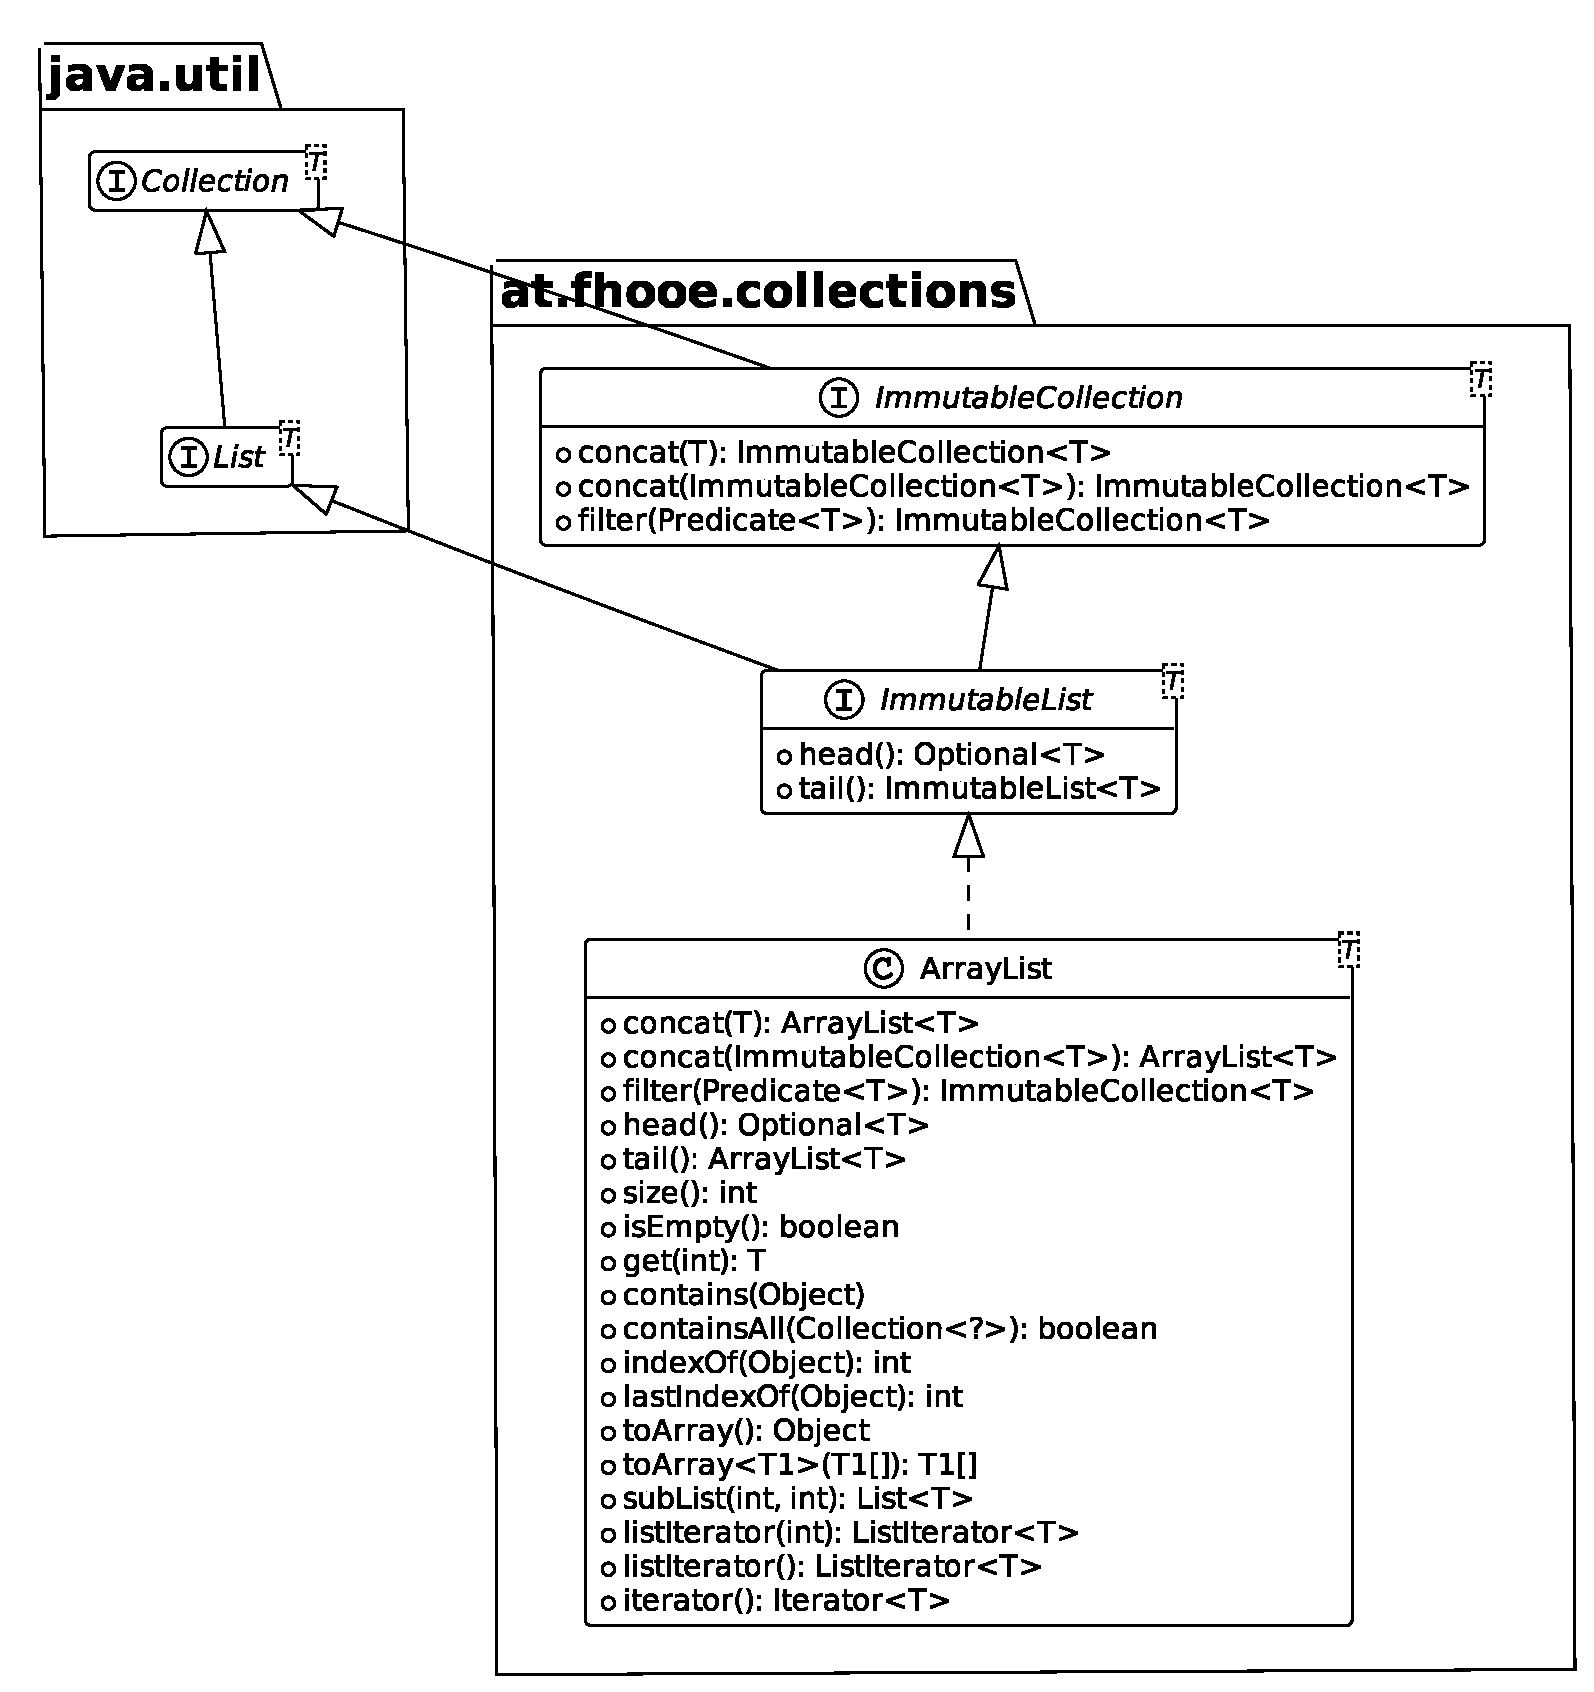
\includegraphics[scale=0.25]{assets/uml/ArrayList-0}
    \label{fig:arraylist-class-diagram}
\end{figure}

\subsection{Developer Experience}\label{subsec:developer-experience}
This subsection describes the developer experience of elegant objects.
By adhering to the elegant object principles, the resulting objects will have a more concise and clearly defined interface.
It also results in code that respects the solid principles, which in turn also make a codebase more maintainable and extensible.

The biggest drawback of using elegant objects with Java is that Java depends heavily on mutable objects.
Therefor, developers using elegant objects have to implement workarounds to limit code where mutable objects are used.
For example the \texttt{Iterator}-interface\footnote{\url{https://docs.oracle.com/en/java/javase/17/docs/api/java.base/java/util/Iterator.html}}, as seen in figure\ \ref{fig:iterator}, is per definition mutable.
The \texttt{next())}-method returns the next element in the iteration.
This means an iterator has to depend on an internal state the changes for each iteration.
For the sake of using only elegant object principle where ever possible an immutable iterator is used, which can be adapted to a Java iterator.
This decision required additional work and implementing an adapter only to meet the elegant object principles.
It also limited all mutable code to only a few classes, which made the rest easier to test and read.
In the end the restriction of mutable objects to specific classes increased the readability of the codebase.
As developers can be sure, if an object is successfully constructed its state is valid.

\begin{figure}[h]
    \caption{Iterator Interface}
    \lstinputlisting[language=Java,basicstyle=\tiny,label={lst:iterator}]{assets/code/Iterator.java}
    \label{fig:iterator}
\end{figure}

Tests are more readable by using immutable objects.
The state of an object can be verified, since every method call will return a new object.
The tests are easier to read, since there is only one assert statement.
It made it clear what part of an object is tested.


    \bibliographystyle{IEEEtran}
    \bibliography{main}

\end{document}
